\documentclass[11pt,a4paper]{ivoa}
\input tthdefs

\usepackage[utf8]{inputenc}

\title{VOSpace}

\ivoagroup{Grid and Web Services Working Group}

\author{Matthew Graham}
\author{Dave Morris}
\author{Guy Rixon}
\author{Pat Dowler}
\author{Andre Schaaff}
\author{Doug Tody}
\author{Brian Major}

\editor{Matthew Graham}
\editor{Brian Major}

\previousversion[http://www.ivoa.net/Documents/WD/GWS/REC-VOSpace-2.0-20130329.html]{REC-VOSpace-2.0-20130329}
\previousversion[http://www.ivoa.net/Documents/WD/GWS/PR-VOSpace-2.0-20121221.html]{PR-VOSpace-2.0-20121221}
\previousversion[http://www.ivoa.net/Documents/WD/GWS/PR-VOSpace-2.0-20120824.html]{PR-VOSpace-2.0-20120824}
\previousversion[http://www.ivoa.net/Documents/WD/GWS/PR-VOSpace-2.0-20111202.html]{PR-VOSpace-2.0-20111202}
\previousversion[http://www.ivoa.net/Documents/WD/GWS/WD-VOSpace-2.0-20110628.html]{WD-VOSpace-2.0-20110628}
\previousversion[http://www.ivoa.net/Documents/WD/GWS/WD-VOSpace-2.0-20101112.html]{WD-VOSpace-2.0-20101112}
\previousversion[http://www.ivoa.net/Documents/GWS/WD-VOSpace-2.0-20100323.html]{WD-VOSpace-2.0-20100323}
\previousversion[http://www.ivoa.net/Documents/GWS/WD-VOSpace-2.0-20090904.html]{WD-VOSpace-2.0-20090904}
\previousversion[http://www.ivoa.net/Documents/GWS/WD-VOSpace-2.0-20090513.doc]{WD-VOSpace-2.0-20090513}
       
\begin{document}
\begin{abstract}
VOSpace is the IVOA interface to distributed storage. This specification presents the second RESTful version of the interface.  Except for minor additions to the 2.1 specification, it is functionally equivalent to the SOAP-based VOSpace 1.1 specification. Note that all 1.x VOSpace clients will not work with this new version of the interface.  Clients and services written for VOSpace 2.1 will interoperate with 2.0 clients and services, however 2.0 clients and services are incompatible with the 2.1 specification.
\end{abstract}

\section*{Acknowledgments}
This document derives from discussions among the Grid and Web Services working group of the IVOA.

This document has been developed with support from the National Science Foundation's Information Technology Research Program under Cooperative Agreement AST0122449 with the John Hopkins University, from the UK Science and Technology Facilities Council (STFC), and from the European Commission's Sixth Framework Program via the Optical Infrared Coordination Network (OPTICON).

\section*{Conformance-related definitions}
The words ``MUST'', ``SHALL'', ``SHOULD'', ``MAY'', ``RECOMMENDED'', and
``OPTIONAL'' (in upper or lower case) used in this document are to be
interpreted as described in IETF standard, \citet{std:RFC2119}.

The \emph{Virtual Observatory (VO)} is
general term for a collection of federated resources that can be used
to conduct astronomical research, education, and outreach.
The \href{http://www.ivoa.net}{International
Virtual Observatory Alliance (IVOA)} is a global
collaboration of separately funded projects to develop standards and
infrastructure that enable VO applications.

\section{Introduction}
VOSpace is the IVOA interface to distributed storage. It specifies how VO agents and applications can use network attached data stores to persist and exchange data in a standard way.

A VOSpace web service is an access point for a distributed storage network. Through this access point, a client can:

add or delete data objects
manipulate metadata for the data objects
obtain URIs through which the content of the data objects can be accessed
VOSpace does not define how the data is stored or transferred, only the control messages to gain access. Thus, the VOSpace interface can readily be added to an existing storage system.

When we speak of "a VOSpace", we mean the arrangement of data accessible through one particular VOSpace service.

Each data object within a VOSpace service is represented as a node and has a description called a representation. A useful analogy to have in mind when reading this document is that a node is equivalent to a file.

Nodes in VOSpace have unique identifiers expressed as URIs in the 'vos' scheme, as defined below.

VOSpace 2.0 did not introduce any new functionality to that already offered by prior (SOAP-based) versions of the interface (VOSpace 1.1) but defines a RESTful binding for the interface. VOSpace 2.1 introduces minor functional changes to VOSpace 2.0 addressing access control and optimizations.

\subsection{Typical use of a VOSpace service}
A typical use case for VOSpace is uploading a local data file to a remote VOSpace service. This is a two-stage process: creating a description of the data file (representation) in the VOSpace including any metadata (its properties) that they want to associate with it (e.g., MIME type), and defining the transfer operation that will actually see the data file bytes uploaded to the VOSpace service. The order of the processes should not matter. The user may want to create the representation first and then perform the transfer or transfer the bytes first and then update the representation with the appropriate metadata.

Let's consider the first sequence: the user provides a XML description of the data file which they HTTP PUT to the appropriate VOSpace URI - this will be the HTTP identifier for the data file in the VOSpace, e.g. http://nvo.caltech.edu/vospace/nodes/mytable1. The description will resemble this:

\begin{verbatim}
<node xmlns="http://www.ivoa.net/xml/VOSpaceTypes-v2.1"
    xmlns:xsi="http://www.w3.org/2001/XMLSchema-instance" 
    uri="vos://nvo.caltech!vospace/mytable1"
    xsi:type="vost:UnstructuredDataNode">  
    <properties> 
        <property uri="ivo://ivoa.net/vospace/core#mimetype">text/xml</property>     
    </properties> 
</node> 
\end{verbatim}

The service will reply with an amended version of the representation containing service-specific details in addition to the information supplied by the user. These will include data formats that the service can handle for the type of node created in the VOSpace, third-party interfaces (capabilities) to the data that the service offers and system metadata.

The user will then describe the data format (the view) they want to use in uploading the file, e.g. VOTable, and the transport protocol (the protocol) that they want to employ to upload the file, e.g. HTTP PUT. This will result in the HTTP POSTing of a XML description of the transfer request to the appropriate VOSpace URI, e.g. http://nvo.caltech.edu/vospace/myData/table123/transfers. The description will resemble this:

\begin{verbatim}
<transfer xmlns="http://www.ivoa.net/xml/VOSpace/v2.1">
    <target>vos://nvo.caltech!vospace/mytable1</target>
    <direction>pushToVoSpace</direction> 
    <view uri="ivo://ivoa.net/vospace/core#votable"/> 
    <protocol uri="ivo://ivoa.net/vospace/core#http-put"/>  
</transfer>
\end{verbatim}

will then use a regular HTTP client to transfer (PUT) the local file to the specified endpoint. This illustrates an important point about VOSpace - it is only concerned with the server-side management of data storage and transfer. A client negotiates the details of a data transfer with a VOSpace service but the actual transfer of bytes across a network is handled by other tools.

Similarly, when a user wants to retrieve a data file from a VOSpace service, they will specify the data format (view) they want to use in downloading the file, e.g. VOTable, and the transport protocol (the protocol) that they want to employ to download the file, e.g. HTTP GET, and HTTP POST a XML description of this transfer request to the appropriate VOSpace URI - the transfer URI for the node in the VOSpace, e.g. http://nvo.caltech.edu/vospace/myDataNode/table123/transfers. The description will resemble this:

\begin{verbatim}
<transfer xmlns="http://www.ivoa.net/xml/VOSpace/v2.1">
    <target>vos://nvo.caltech!vospace/mytable1</target>
    <direction>pullFromVoSpace</direction> 
    <view uri="ivo://ivoa.net/vospace/core#votable"/> 
    <protocol uri="ivo://ivoa.net/vospace/core#httpget"/>  
</transfer>
\end{verbatim}

The service will reply with the URL for the user to use, e.g. http://nvo.caltech.edu/vospace/myDataNode/table123/transfers/3df89ab4. The user can then download the data file by pointing an HTTP client (e.g. web browser) at the specified endpoint.

\subsection{Role within the VO Architecture}

The IVOA Architecture [Arch] provides a high-level view of how IVOA standards work together to connect users and applications with providers of data and services, as depicted in the diagram in Figure ~\ref{fig:archdiag}.

\begin{figure}
\centering

% Get the architecture diagram from the TCG chair
% http://wiki.ivoa.net/twiki/bin/view/IVOA/IvoaTCG
% If they give you a PDF, for now dumb it down to a png by
% convert -antialias -density 72x72 archdiag.pdf archdiag.png
% Oh -- Notes don't need this; you'd have to remove archdiag.png
% from FIGURES in the Makefile, too.

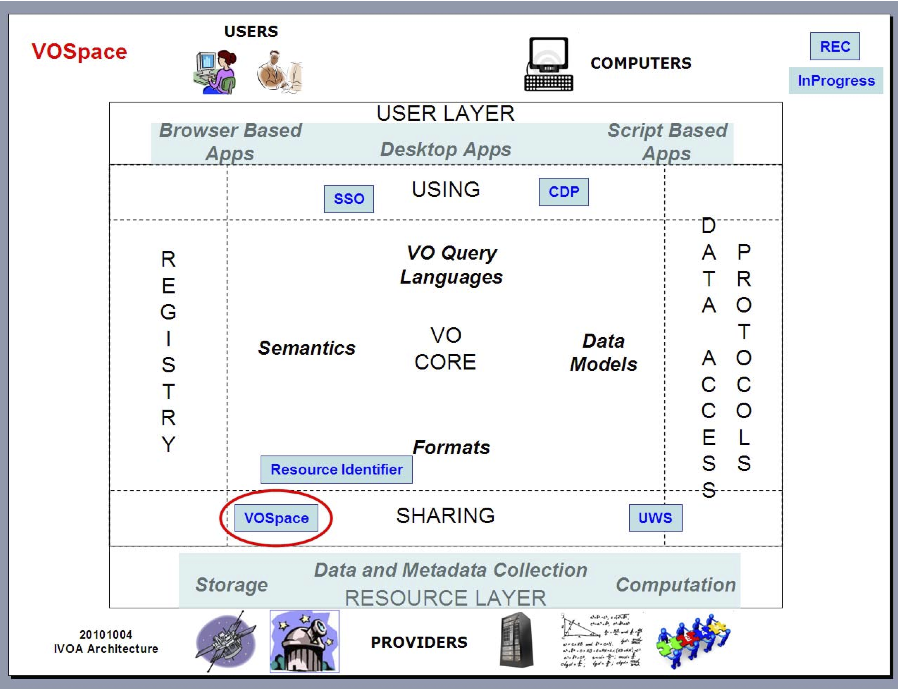
\includegraphics[width=0.9\textwidth]{archdiag.png}
\caption{VOSpace in the IVOA Architecture. This provides an interface to distributed storage. It specifies how applications can use networked data stores to persist and exchange data in a standardized fashion.}
\label{fig:archdiag}
\end{figure}

In this architecture, users employ a variety of tools (from the User Layer) to discover and access archives and services of interest (represented in the Resource Layer). VOSpace provides an interface to storage resources containing the results of using these archives and services and also to other storage solutions, e.g., local disks, where users might want to transfer these results for further work. Items in these resources are referenced by a VOSpace identifier which is related to the standard IVOA Resource Identifier (see section 2). This version of VOSpace employs the UWS design pattern [UWS] to manage data transfers (see section 3.6) and searches (see section 3.7). VOSpace instances may also employ the IVOA Single-Sign-On standard [SSO] for authentication purposes (see section 4) and IVOA Credential Delegation Protocol [CDP] to delegate data transfers.

\subsection{Document roadmap}
The rest of this document is structured as follows:

In Section 2 (TODO: link these section references), we specify the URI syntax for identifying data objects (nodes) in VOSpace.

In Section 3, we present the data model that underpins the VOSpace architecture. This consists of a number of data structures, which have XML representations that are used across the wire in message exchanges with a VOSpace service. These structures represent:

the data objects themselves (nodes)
metadata that can be associated with a data object (properties)
third-party interfaces to the data (capabilities)
the data format used when transferring data objects across the wire (views)
the transport protocol employed in a data transfer (protocols)
the data transfer itself (transfers)
searches of data objects (searches)
We also describe the REST bindings between these representations and their URIs (HTTP identifiers).

In Section 4, we outline how security and access control policies are currently handled in VOSpace.

In Section 5, we detail the operations that the VOSpace interface supports. These handle access to service-level metadata, the creation and manipulation of nodes within the VOSpace, access to node metadata (properties) and data transfer to and from the VOSpace.

In Appendix A, we formally define the VOSpace interface with a machine readable description of its requests and responses and in Appendix B, we present a compliance matrix listing the mandatory behaviour required of a valid VOSpace 2.1 service.

\section{VOSpace identifiers}
The identifier for a node in VOSpace SHALL be a URI with the scheme vos.

Such a URI SHALL have the following parts with the meanings and encoding rules defined in RFC2396 [TODO].

\begin{itemize}
  \item scheme
  \item naming authority
  \item path
  \item (optional) query
  \item (optional) fragment identifier (with the expected semantics [TODO])
\end{itemize}

The naming authority for a VOSpace node SHALL be the VOSpace service through which the node was created. The authority part of the URI SHALL be constructed from the IVO registry identifier [IVORN] for that service by deleting the ivo:// prefix and changing all forward-slash characters('/') in the resource key to exclamation marks ('!') or tildes ('~'). Note that a service SHALL be consistent in its use of separator characters ('!' or '~') when referring to its own data but SHALL accept either as valid in URIs in service requests. For the rest of the document, we shall use '!' as the default character.

This is an example of a possible VOSpace identifier.

\begin{verbatim}
vos://nvo.caltech!vospace/myresults/siap-out-1.vot
\end{verbatim}

The URI scheme is \emph{vos}

Using a separate URI scheme for VOSpace identifiers enables clients to distinguish between IVO registry identifiers and VOSpace identifiers.

\begin{itemize}
    \item nvo.caltech!vospace
\end{itemize}

is the authority part of the URI, corresponding to the IVO registry identifier

\begin{itemize}
    \item ivo://nvo.caltech/vospace
\end{itemize}

This is the IVO registry identifier of the VOSpace service that contains the node.

\begin{itemize}
    \item /siap-out-1.vot is the URI path
\end{itemize}

Slashes in the URI path imply a hierarchical arrangement of data: the data object identified by vos://nvo.caltech!vospace/myresults/siap-out-1.vot is within the container identified by vos://nvo.caltech!vospace/myresults.

Literal space characters are also not allowed in URIs.

All ancestors in the hierarchy SHALL be resolvable as containers (ContainerNodes), all the way up to the root node of the space (this precludes any system of implied hierarchy in the naming scheme for nodes with ancestors that are just logical entities and cannot be reified, e.g. the Amazon S3 system).

A VOSpace identifier is globally unique, and identifies one specific node in a specific VOSpace service.

The standardID for this specification SHALL be: ivo://ivoa.net/std/VOSpace/v2.1.

\subsection{Identifier resolution}
A VOSpace identifier can be resolved to a HTTP endpoint for accessing representations of the node associated with it. A client SHOULD use the following procedure to resolve access to a VOSpace node from a VOSpace identifier:

\begin{itemize}
    \item Resolve HTTP service endpoint of VOSpace service with registry
    \item Append "nodes/" and the path following the naming authority part of the VOSpace identifier to the service endpoint
\end{itemize}

Given the example identifier

\begin{verbatim}
    vos://org.astrogrid.cam!vospace/container-6/siap-out-1.vot?foo=bar
\end{verbatim}

processing the URI to resolve the VOSpace service would involve :

\begin{enumerate}
    \item Extract the IVO registry identifier of the VOSpace service by prepending an ivo scheme to the naming authority part:
        \begin{verbatim}
            ivo://org.astrogrid.cam/vospace
        \end{verbatim}
    \item Resolve the IVO identifier in a registry and retrieve the access URL of the service endpoint:
        \begin{verbatim}
            http://some.uni.ac.uk/vospace
        \end{verbatim}
    \item Append "nodes/" and the path part of the VOSpace identifier:
        \begin{verbatim}
            http://some.uni.ac.uk/vospace/nodes/container-6/siap-out-1.vot?foo=bar
        \end{verbatim}
\end{enumerate}

Note that any fragment identifier in the identifier SHOULD be removed when resolving the identifier to a HTTP endpoint, consistent with the implied semantics of URI fragments [TODO].

\section{VOSpace data model}

\subsection{Nodes and node types}

We refer to the arrangement of data accessible through one particular VOSpace service as "a VOSpace".

Each data object within a VOSpace SHALL be represented as a node that is identified by a URI.

There are different types of nodes and the type of a VOSpace node determines how the VOSpace service stores and interprets the node data.

The types are arranged in a hierarchy (see Figure ~\ref{fig:nodehierarchy}), with more detailed types inheriting the structure of more generic types.

\begin{figure}
\centering
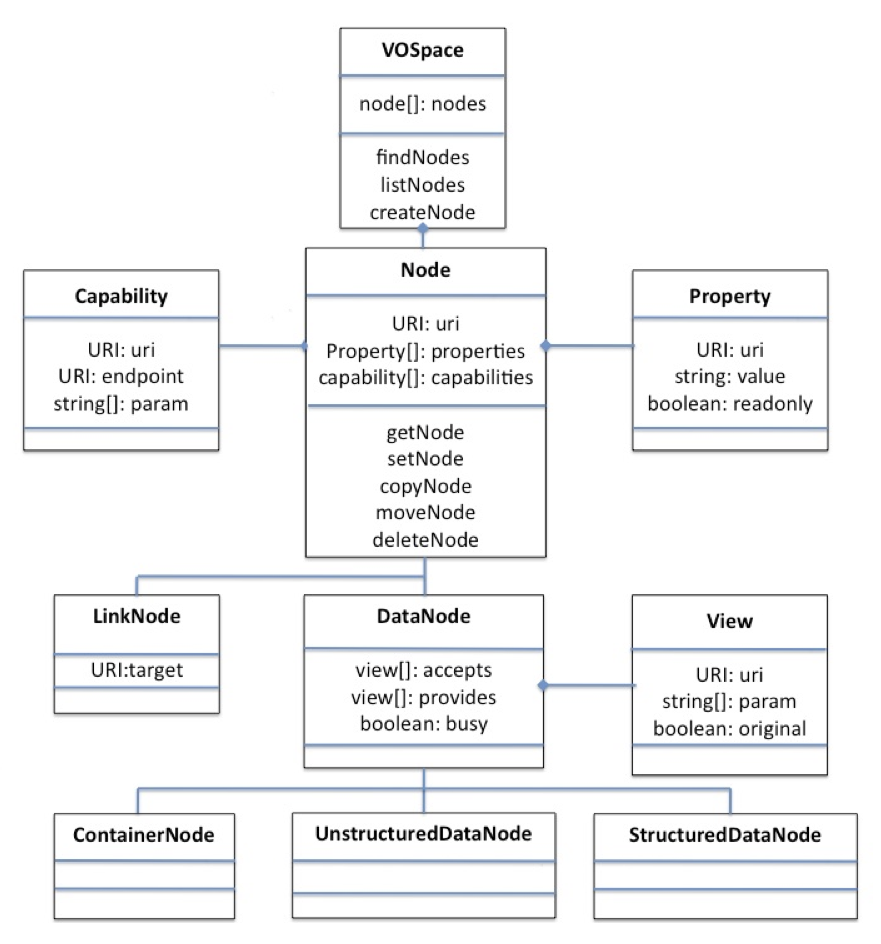
\includegraphics[width=0.9\textwidth]{vospace-node-hierarchy.png}
\caption{Node hierarchy - This shows the inheritance structure for the different types of nodes in VOSpace.}
\label{fig:nodehierarchy}
\end{figure}

The following types (and representations) are defined:

\begin{itemize}
    \item Node is the most basic type
    \item ContainerNode describes a data item that can contain other data items
    \item DataNode describes a data item stored in the VOSpace
    \item UnstructuredDataNode describes a data item for which the VOSpace does not understand the data format
    \item StructuredDataNode describes a data item for which the space understands the format and may make transformations that preserve the meaning of the data.
    \item LinkNode describes a node that points to another node.
\end{itemize}

When data is stored and retrieved from an \emph{UnstructuredDataNode}, the bit pattern read back SHALL be identical to that written.

When data is stored and retrieved from a \emph{StructuredDataNode}, the bit pattern returned MAY be different to the original. For example, storing tabular data from a VOTable file will preserve the tabular data, but any comments in the original XML file may be lost.

A Node representation SHALL have the following elements:

\begin{itemize}
    \item \emph{uri}: the vos:// identifier for the node, URI-encoded according to RFC2396 [TODO]
    \item \emph{properties}: a set of metadata properties for the node
    \item \emph{capabilities}: a third-party interface to a data object
\end{itemize}

In addition, a \emph{DataNode} representation SHALL have the following elements:

\begin{itemize}
    \item \emph{accepts}: a list of the views (data formats) that the node can accept
    \item \emph{provides}: a list of the views (data formats) that the node can provide
    \item \emph{busy}: a boolean flag to indicate that the data associated with the node cannot be accessed
\end{itemize}

The \emph{busy} flag is used to indicate that an internal operation is in progress, and the node data is not available.

A \emph{ContainerNode} representation SHALL have the following elements, in addition to those it inherits from the \emph{Node} representation:

\begin{itemize}
    \item \emph{nodes}: a list of the direct children, if applicable, that the container has. Each child is represented as a node subelement containing its vos:// identifier, URI-encoded according to RFC2396 [TODO]
\end{itemize}

A \emph{LinkNode} representation SHALL have the following elements, in addition to those it inherits from the Node representation:

\begin{itemize}
    \item \emph{target}: the target URI, URI-encoded according to RFC2396 [TODO]
\end{itemize}

The link target can be a URI that points to any type of resource, including other VOSpace Nodes (within the same VOSpace service or in another service), or external resources outside VOSpace altogether.

The properties of a \emph{LinkNode} do not propagate to the target of the \emph{LinkNode}, i.e., a property attached to a LinkNode does not also get attached to the target node. One use case is to enable third-party annotations to be associated with a resource but without the resource itself getting cluttered with unnecessary metadata. In this case, the client creates a \emph{LinkNode} pointing to the resource in question and then adds the annotations as properties of the \emph{LinkNode}.

Both the \emph{ContainerNode} and the \emph{LinkNode} SHALL have no data bytes associated with them.

The set of node types defined by this standard is closed; new types may be introduced only via new versions of the standard.

To comply with the standard, a client or service SHALL be able to parse XML representations of all the node types defined in the current specification.

Note: This does not require all services to support all of the Node types, just that it can process an XML request containing any of the types. If the service receives a request for a type that it does not support, the service SHOULD return a \emph{TypeNotSupported} fault. The service SHALL NOT throw an XML parser error if it receives a request for a type that it does not support.

\subsection{Properties}
\emph{Properties} are simple string-based metadata properties associated with a node.

Individual \emph{Properties} should contain simple short string values, not large blocks of information. If a system needs to attach a large amount of metadata to a node, then it should either use multiple small \emph{Properties}, or a single \emph{Property} containing a URI or URL pointing to an external resource that contains the additional metadata.

A \emph{Property} representation SHALL have the following elements:

\begin{itemize}
    \item \emph{uri}: the Property identifier
    \item \emph{value}: the string value of the Property
    \item \emph{readOnly}: a boolean flag to indicate that the Property cannot be changed by the client
\end{itemize}

Properties may be set by the client or the service.

\subsubsection{Property values}
Unless they have special meaning to the service or client, Properties are treated as simple string values.

When a \emph{Property} can take multiple values, e.g., a list of groups which can access a particular resource, these SHOULD be comma-separated, unless the property description defines a specific delimiter.

Some \emph{Properties} may have meaning to the service; others may have meaning only to one specific type of client. A service implementation does not need to understand the meaning of all the \emph{Properties} of a node. Any Properties that it does not understand can simply be stored as text strings.

\subsubsection{Property identifiers}
Every new type of \emph{Property} SHALL require a unique URI to identify the \emph{Property} and its meaning.

The rules for the \emph{Property} identifiers are similar to the rules for namespace URIs in XML schema. The only restriction is that it SHALL be a valid (unique) URI.

\begin{itemize}
    \item An XML schema namespace identifier can be just a simple URN, e.g. urn:my?namespace
    \item Within the IVOA, the convention for namespace identifiers is to use a HTTP URL pointing to the namespace schema or a resource describing it
\end{itemize}

The current VOSpace schema defines \emph{Property} identifiers as anyURI. The only restriction is that it SHALL be a valid (unique) URI.

\begin{itemize}
    \item A \emph{Property} URI can be a simple URN, e.g. urn:my?property
\end{itemize}

This may be sufficient for testing and development on a private system, but it is not scalable for use on a public service.

For a production system, any new Properties SHOULD have unique URIs that can be resolved into to a description of the Property.

Ideally, these should be IVO registry URIs that point to a description registered in the IVO registry:

\begin{itemize}
    \item ivo://my?registry/vospace/properties\#my?property
\end{itemize}

Using an IVO registry URI to identify Properties has two main advantages:

\begin{itemize}
    \item IVO registry URIs are by their nature unique, which makes it easy to ensure that different teams do not accidentally use the same URI
    \item If the IVO registry URI points to a description registered in the IVO registry, this provides a mechanism to discover what the Property means
\end{itemize}

\subsubsection{Property descriptions}
If the URI for a particular Property is resolvable, i.e. an IVO registry identifier or a HTTP URL, then it SHOULD point to an XML resource that describes the Property.

A Property description SHOULD describe the data type and meaning of a Property.

A PropertyDescription SHOULD have the following members:

\begin{itemize}
    \item \emph{uri}: the formal URI of the Property
    \item \emph{DisplayName}: A display name for the Property
    \item \emph{Description}: A text block describing the meaning and validation rules of the Property
\end{itemize}

A PropertyDescription MAY have the following OPTIONAL members:

\begin{itemize}
    \item \emph{UCD}: the Universal Content Descriptor (in the UCD1+ scheme) for the Property
    \item \emph{Unit}: the unit of measurement of the Property
\end{itemize}

The information in a Property description can be used to generate a UI for displaying and modifying the different types of Properties.

Note that at the time of writing, the schema for registering PropertyDescriptions in the IVO registry has not been finalized.

\paragraph{UI Display name}
If a client is unable to resolve a Property identifier into a description, then it may just display the identifier as a text string:

\begin{itemize}
    \item urn:modifieddate
\end{itemize}

If the client can resolve the Property identifier into a description, then the client may use the information in the description to display a human readable name and description of the Property:

\begin{itemize}
    \item Last modification date of the node data
\end{itemize}

\paragraph{Property editors}
If the client is unable to resolve a Property identifier into a description, or does not understand the type information defined in the description, then the client MAY treat the Property value as a simple text string.

If the client can resolve the Property identifier into a description, then the client MAY use the information in the description to display an appropriate editing tool for the Property.

In the current version of the specification the rules for editing Properties are as follows:

\begin{itemize}
    \item A service MAY impose validation rules on the values of specific types of Properties
    \item If a client attempts to set a Property to an invalid value, then the service MAY reject the change
    \item Where possible, the validation rules for a type of Property SHOULD be defined in the Property description
\end{itemize}

Future versions of the VOSpace specification may extend the PropertyDescription to include more specific machine readable validation rules for a Property type.

Note that at the time of writing, the schema for registering validation rules in PropertyDescriptions has not been finalized.

\subsubsection{Standard properties}
Property URIs and PropertyDescriptions for the core set of Properties are registered under a StandardKeyEnumeration resource [VOStd] in the IVOA registry with the resource identifier ivo://ivoa.net/vospace/core. The following URIs SHOULD be used to represent the service properties:

\begin{itemize}
    \item ivo://ivoa.net/vospace/core\#title SHALL be used as the property URI denoting a name given to the resource
    \item ivo://ivoa.net/vospace/core\#creator SHALL be used as the property URI denoting an entity primarily responsible for making the resource
    \item ivo://ivoa.net/vospace/core\#subject SHALL be used as the property URI denoting the topic of the resource
    \item ivo://ivoa.net/vospace/core\#description SHALL be used as the property URI denoting an account of the resource
    \item ivo://ivoa.net/vospace/core\#publisher SHALL be used as the property URI denoting an entity responsible for making the resource available
    \item ivo://ivoa.net/vospace/core\#contributor SHALL be used as the property URI denoting an entity responsible for making contributions to this resource
    \item ivo://ivoa.net/vospace/core\#date SHALL be used as the property URI denoting a point or period of time associated with an event in the lifecycle of the resource
    \item ivo://ivoa.net/vospace/core\#type SHALL be used as the property URI denoting the nature or genre of the resource
    \item ivo://ivoa.net/vospace/core\#format SHALL be used as the property URI denoting the file format, physical medium, or dimensions of the resource
    \item ivo://ivoa.net/vospace/core\#identifier SHALL be used as the property URI denoting an unambiguous reference to the resource within a given context
    \item ivo://ivoa.net/vospace/core\#source SHALL be used as the property URI denoting a related resource from which the described resource is derived
    \item ivo://ivoa.net/vospace/core\#language SHALL be used as the property URI denoting a language of the resource
    \item ivo://ivoa.net/vospace/core\#relation SHALL be used as the property URI denoting a related resource
    \item ivo://ivoa.net/vospace/core\#coverage SHALL be used as the property URI denoting the spatial or temporal topic of the resource, the spatial applicability of the resource, or the jurisdiction under which the resource is relevant
    \item ivo://ivoa.net/vospace/core\#rights SHALL be used as the property URI denoting information about rights held in and over the resource
    \item ivo://ivoa.net/vospace/core\#availableSpace SHALL be used as the property URI denoting the amount of space available within a container
    \item ivo://ivoa.net/vospace/core\#groupread SHALL be used as the property URI denoting the list of groups which can only read this resource (read-only)
    \item ivo://ivoa.net/vospace/core\#groupwrite SHALL be used as the property URI denoting the list of groups which can read and write to this resource (read-write)
    \item ivo://ivoa.net/vospace/core\#publicread SHALL be used as the property URI denoting whether this resource is world readable (anon-read-only)
    \item ivo://ivoa.net/vospace/core\#quota SHALL be used as the property URI denoting the value of a system quota on the resource
    \item ivo://ivoa.net/vospace/core\#length SHALL be used as the property URI denoting the length or size of a resource
    \item ivo://ivoa.net/vospace/core\#mtime SHALL be used as the property URI denoting the data modification time
    \item ivo://ivoa.net/vospace/core\#ctime SHALL be used as the property URI denoting status change (aka metadata modification) time
    \item ivo://ivoa.net/vospace/core\#btime SHALL be used as the property URI denoting initial creation time
\end{itemize}

However, this is not intended to be a closed list, different implementations are free to define and use their own Properties.

\subsection{Capabilities}
A Capability describes a third-party interface to a node. One application of this would be to enable data access to a node or its contents using a 3rd party service interface.

A Capability representation SHALL have the following members:

\begin{itemize}
    \item \emph{uri}: the Capability identifier
    \item \emph{endpoint}: the endpoint URL to use for the third-party interface
    \item \emph{param}: a set of parameters for the capability
\end{itemize}

\subsubsection{Example use cases}
A ContainerNode containing image files may offer a DAL SIAP capability so that the images in the container can be accessed using a SIAP service. In this way, a user could create a (DAL enabled) Container in VOSpace, transfer some images into it and then query the set of images using the SIAP interface.

Another example is a DataNode that provides an iRODS capability so that the data replication for this data object can be handled using the iRODS service API.

\subsubsection{Capability identifiers}
Every new type of Capability SHALL require a unique URI to identify the Capability. The rules for the Capability identifiers are similar to the rules for namespace URIs in XML schema. The only restriction is that it SHALL be a valid (unique) URI.

\begin{itemize}
    \item An XML schema namespace identifier can be just a simple URN, e.g. urn:my-namespace
    \item Within the IVOA, the convention for namespace identifiers is to use a HTTP URL pointing to the namespace schema, or a resource describing it.
\end{itemize}

The VOSpace schema defines Capability identifiers as anyURI. The only restriction is that it SHALL be a valid (unique) URI.

\begin{itemize}
    \item A Capability URI can be a simple URN, e.g. urn:my-capability
\end{itemize}

This may be sufficient for testing and development on a private system, but it is not suitable for use on a public service. For a production system, any new Capabilities SHOULD have unique URIs that can be resolved into a description of the Capability. Ideally, these SHOULD be IVO registry URIs that point to a description registered in the IVO registry:

\begin{itemize}
    \item ivo://my-registry/vospace/capabilities\#my-capability
\end{itemize}

Using an IVO registry URI to identify Capabilities has two main advantages:

\begin{itemize}
    \item IVO registry URIs are by their nature unique, which makes it easy to ensure that different teams do not accidentally use the same URI
    \item If the IVO registry URI points to a description registered in the IVO registry, this provides a mechanism to discover how to use the Capability.
\end{itemize}

\subsubsection{Capability descriptions}
If the URI for a particular Capability is resolvable, i.e. an IVO registry identifier or a HTTP URL then it SHOULD point to an XML resource that describes the Capability.

A CapabilityDescription SHOULD describe the third-party interface and how it should be used in this context. A CapabilityDescription SHOULD have the following members:

\begin{itemize}
    \item \emph{uri}: the formal URI of the Capability
    \item \emph{DisplayName}: a simple display name of the Capability.
    \item \emph{Description}: a text block describing the third-party interface and how it should be used in this context.
\end{itemize}

Note that at the time of writing, the schema for registering CapabilityDescriptions in the IVO registry has not been finalized.

\subsubsection{UI display name}
If a client is unable to resolve a Capability identifier into a description then it may just display the identifier as a text string:

\begin{itemize}
    \item Access data using urn:edu.sdsc.irods
\end{itemize}

If a client can resolve the Capability identifier into a description then the client may use the information in the description to display a human readable name and description of the Capability:

\begin{itemize}
    \item Access data using iRODS
\end{itemize}

\subsubsection{Standard capabilities}
Capability URIs and CapabilityDescriptions for the core set of Capabilities are registered under a StandardKeyEnumeration resource [VOStd] in the IVOA registry with the resource identifier ivo://ivoa.net/vospace/core.. The following URIs SHALL be used to represent the service capabilities:

\begin{itemize}
    \item ivo://ivoa.net/vospace/core\#vospace-1.0 SHALL be used as the capability URI for a VOSpace 1.0 service
    \item ivo://ivoa.net/vospace/core\#vospace-1.1 SHALL be used as the capability URI for a VOSpace 1.1 service
    \item ivo://ivoa.net/vospace/core\#vospace-2.0 SHALL be used as the capability URI for a VOSpace 2.0 service
\end{itemize}
If a service implementation supports more than one version of the VOSpace interface then these capability URIs can be used with a VOSpace service to identify different VOSpace capabilities for a node.

One use case for this would be a VOSpace 1.1 client talking to a service that implements both VOSpace 1.0 and VOSpace 1.1, where the client is acting on behalf of a third party agent that only understands VOSpace 1.0. In this case, the client can use the information in the VOSpace 1.0 capability to direct the third party agent to the VOSpace 1.0 endpoint.

Other standard service interfaces will also be registered, e.g.

\begin{itemize}
    \item Cone Search
    \item SIAP
    \item SSAP
    \item TAP
\end{itemize}

However, this is not intended to be a closed list and different implementations are free to define and use their own Capabilities.

\subsection{Views}
A View describes the data formats and contents available for importing or exporting data to or from a VOSpace node.

The metadata for a DataNode contains two lists of Views.

\begin{itemize}
    \item \emph{accepts}: is a list of Views that the service can accept for importing data into the Node
    \item \emph{provides}: is a list of Views that the service can provide for exporting data from Node
\end{itemize}

A View representation SHALL have the following members:

\begin{itemize}
    \item \emph{uri}: an optional boolean flag to indicate that the View preserves the original bit pattern of the data
    \item \emph{original}: a set of name-value pairs that can be used to specify additional arguments for the View
\end{itemize}

\subsubsection{Example use cases}
A simple VOSpace system that stores data as a binary files can just return the contents of the original file. The client supplies a View identifier when it imports the data, and the service uses this information to describe the data to other clients.

A file based system can use the special case identifier 'ivo://ivoa.net/vospace/core\#view?any' to indicate that it will accept any data format or View for a Node.

For example:

\begin{itemize}
    \item A client imports a file into the service, specifying a View to describe the file contents
    \item The service stores the data as a binary file and keeps a record of the View
    \item The service can then use the View supplied by the client to describe the data to other clients
\end{itemize}

This type of service is not required to understand the imported data, or to verify that it contents match the View, it treats all data as binary files.

\paragraph{Database store}
A VOSpace system that stores data in database tables would need to be able to understand the data format of an imported file in order to parse the data and store it correctly. This means that the service can only accept a specific set of Views, or data formats, for importing data into the Node.

In order to tell the client what input data formats it can accept, the service publishes a list of specific Views in the accepts list for each Node.

On the output side, a database system would not be able to provide access to the original input file. The contents of file would have been transferred into the database table and then discarded. The system has to generate the output results from the contents of the database table.

In order to support this, the service needs to be able to tell the client what Views of the data are available.

A database system may offer access to the table contents as either VOTable or FITS files, it may also offer zip or tar.gz compressed versions of these. In which case the system needs to be able to express nested file formats such as 'zip containing VOTable' and 'tar.gz containing FITS'.

A service may also offer subsets of the data. For example, a work flow system may only want to look at the table headers to decide what steps are required to process the data. If the table contains a large quantity of data, then downloading the whole contents just to look at the header information is inefficient. To make this easier, a database system may offer a 'metadata only' View of the table, returning a VOTable or FITS file containing just the metadata headers and no rows.

So our example service may want to offer the following Views of a database table:

\begin{itemize}
    \item Table contents as FITS
    \item Table contents as VOTable
    \item Table contents as zip containing FITS
    \item Table contents as zip containing VOTable
    \item Table contents as tar.gz containing FITS
    \item Table contents as tar.gz containing VOTable
    \item Table metadata as FITS
    \item Table metadata as VOTable
\end{itemize}

The service would publish this information as a list of Views in the provides section of the metadata for each Node.

The VOSpace specification does not mandate what Views a service must provide. The VOSpace specification is intended to provide a flexible mechanism enabling services to describe a variety of different Views of data. It is up to the service implementation to decide what Views of the data it can accept and provide.

\subsubsection{View identifiers}
Every new type of View SHALL require a unique URI to identify the View and its content.

The rules for the View identifiers are similar to the rules for namespace URIs in XML schema. The only restriction is that it SHALL be a valid (unique) URI.

\begin{itemize}
    \item An XML schema namespace identifier can be just a simple URN, e.g. urn:my?namespace
    \item Within the IVOA, the convention for namespace identifiers is to use a HTTP URL pointing to the namespace schema, or a resource describing it
\end{itemize}

The current VOSpace schema defines View identifiers as anyURI. The only restriction is that it SHALL be a valid (unique) URI.

\begin{itemize}
    \item A View URI can be a simple URN, e.g. urn:my?view
\end{itemize}

This may be sufficient for testing and development on a private system, but it is not scalable for use on a public service.

For a production system, any new Views SHOULD have unique URIs that can be resolved into to a description of the View.

Ideally, these should be IVO registry URIs that point to a description registered in the IVO registry:

\begin{itemize}
    \item ivo://my?registry/vospace/views\#my?view
\end{itemize}

Using an IVO registry URI to identify Views has two main advantages:

\begin{itemize}
    \item IVO registry URIs are by their nature unique, which makes it easy to ensure that different teams do not accidentally use the same URI
    \item If the IVO registry URI points to a description registered in the IVO registry, this provides a mechanism to discover what the View contains
\end{itemize}

\subsubsection{View descriptions}
If the URI for a particular View is resolvable, i.e. an IVO registry identifier or a HTTP URL, then it SHOULD point to an XML resource that describes the View.

A ViewDescription SHOULD describe the data format and/or content of the view.

A ViewDescription SHOULD have the following members :

\begin{itemize}
    \item \emph{uri}: the formal URI of the View
    \item \emph{DisplayName}: a simple display name of the View.
    \item \emph{Description}: a text block describing the data format and content of the View.
\end{itemize}

A ViewDescription MAY have the following optional members:

\begin{itemize}
    \item \emph{MimeType}: the standard MIME type of the View, if applicable
    \item \emph{Parameters}: a list of required and option parameters the view accepts, if applicable
\end{itemize}

However, at the time of writing, the schema for registering ViewDescriptions in the IVO registry has not been finalized.

\paragraph{UI Display name}
If a client is unable to resolve a View identifier into a description, then it MAY just display the identifier as a text string:

\begin{itemize}
    \item Download as urn:table.meta.fits
\end{itemize}

If the client can resolve the View identifier into a description, then the client MAY use the information in the description to display a human readable name and description of the View:

\begin{itemize}
    \item Download table metadata as FITS header
\end{itemize}

\paragraph{Mime Types}
If a VOSpace service provides HTTP access to the data contained in a Node, then if the ViewDescription contains a MimeType field, this SHOULD be included in the appropriate header field of the HTTP response.

\subsubsection{Default views}
The following standard URIs are registered under a StandardKeyEnumeration resource [VOStd] in the IVOA registry with the resource identifier ivo://ivoa.net/vospace/core. They SHALL be used to refer to the default import and export views:

\begin{itemize}
    \item ivo://ivoa.net/vospace/core\#anyview SHALL be used as the view URI to indicate that a service will accept any view for an import operation
    \item ivo://ivoa.net/vospace/core\#binaryview SHALL be used as the view URI to import or export data as a binary file
    \item ivo://ivoa.net/vospace/core\#defaultview SHALL be used by a client to indicate that the service should choose the most appropriate view for a data export
\end{itemize}

\paragraph{Default import view}
If a client imports data using this view, the data SHALL be treated as a binary BLOB, and stored as is with no additional processing. This is equivalent to the application/binary MIME type.

Note, this view is OPTIONAL, and the service may throw a ViewNotSupported exception if it does not accept this view. In particular, this view cannot be used to import data into a StructuredDataNode as the service needs to know about and understand the data format to be able to create the StructuredDataNode.

Note, this view is only valid for the data import operations, pullToVoSpace and pushToVoSpace. If this view is requested in an export operation, pullFromVoSpace and pushToVoSpace, then the service SHOULD throw a ViewNotSupported exception.

\paragraph{Default export view}
If a client requests data using this view, the server SHALL choose whichever of the available views (the server) thinks is the most appropriate, based on how the data is stored. In a simple file-based system, this will probably be the same format that the data was originally imported in. In a database table system, this will probably either be VOTable or CVS, depending on the level of metadata available.

Note, this view is OPTIONAL, and the server may throw a ViewNotSupported exception if it does not provide this view. However, in most cases, it is expected that a service would be able to select an appropriate 'default' format for data held within the service.

Note, this view is only valid for the data export operations, pullFromVoSpace and pushFromVoSpace. If this view is requested in an import operation, pullToVoSpace and pushToVoSpace, then the service SHOULD throw a ViewNotSupported fault.

\subsubsection{Container views}
In VOSpace 2.1, a view of a ContainerNode describes the data representation (format) of a file or data stream that represents the combined contents of the node and its children. If the view describes an archive format (tar, zip, etc.) then a service that accepts this view (format) for a ContainerNode SHALL provide access to the archive contents as children nodes of the container. Whether or not the service actually unpacks the archive is implementation dependent but the service SHALL behave as though it has done so. For example, a client may want to upload a tar file containing several images to a VOSpace service. If they associate it with (upload it to) a (Un)structuredDataNode then it will be treated as a blob and its contents will be not be available. However, if they upload it to a ContainerNode with an accepts view of "tar" then the image files within the tar file will be represented as children nodes of the ContainerNode and accessible like any other data object within the space.

If a service provides an archive format (tar, zip, etc.) view of a ContainerNode then the service SHALL package the contents of the container and all its child nodes in the specified format.

\subsection{Protocols}
A Protocol describes the parameters required to perform a data transfer using a particular protocol.

A Protocol representation SHALL have the following members:

\begin{itemize}
    \item \emph{uri}: the Protocol identifier
    \item \emph{endpoint}: the endpoint URL to use for the data transfer additional arguments required for the transfer
\end{itemize}

A protocol representation MAY have the following members:

\begin{itemize}
    \item \emph{param}: A list of name-value pairs that specify any additional arguments requried for the transfer
    \item \emph{authType}: The requested type of authentication method to be used
\end{itemize}

Note: endpoint will only contain a value after the response from the service is received.

\subsubsection{Protocol identifiers}
Every new type of Protocol requires a unique URI to identify the Protocol and how to use it.

The rules for the Protocol identifiers are similar to the rules for namespace URIs in XML schema. The only restriction is that it SHALL be a valid (unique) URI

\begin{itemize}
    \item An XML schema namespace identifier can be just a simple URN, e.g. urn:my?namespace
    \item Within the IVOA, the convention for namespace identifiers is to use a HTTP URL pointing to the namespace schema, or a resource describing it
\end{itemize}

The current VOSpace schema defines Protocol identifiers as anyURI. The only restriction is that it SHALL be a valid (unique) URI.

\begin{itemize}
    \item A Protocol URI can be a simple URN, e.g. urn:my?protocol
\end{itemize}

This may be sufficient for testing and development on a private system, but it is not scalable for use on a public service.

For a production system, any new Protocols SHOULD have unique URIs that can be resolved into to a description of the Protocol.

Ideally, these should be IVO registry URIs that point to a description registered in the IVO registry:

\begin{itemize}
    \item \begin{verbatim}ivo://my?registry/vospace/protocols#my?protocol\end{verbatim}
\end{itemize}

Using an IVO registry URI to identify Protocols has two main advantages:

\begin{itemize}
    \item IVO registry URIs are by their nature unique, which makes it easy to ensure that different teams do not accidentally use the same URI
    \item If the IVO registry URI points to a description registered in the IVO registry, this provides a mechanism to discover how to use the Protocol
\end{itemize}

\subsubsection{Protocol descriptions}
If the URI for a particular Protocol is resolvable, i.e. an IVO registry identifier or a HTTP URL, then it SHOULD point to an XML resource that describes the Protocol.

A ProtocolDescription SHOULD describe the underlying transport protocol, and how it should be used in this context.

A ProtocolDescription SHOULD have the following members:

\begin{itemize}
    \item \emph{uri}: the formal URI of the Protocol
    \item \emph{DisplayName}: A simple display name of the Protocol
    \item \emph{Description}: Text block describing describing the underlying transport protocol, and how it should be used in this context
\end{itemize}

However, at the time of writing, the schema for registering ProtocolDescriptions in the IVO registry has not been finalized.

\paragraph{UI display name}

If a client is unable to resolve a Protocol identifier into a description, then it MAY just display the identifier as a text string:

\begin{itemize}
    \item Download using urn:my?protocol
\end{itemize}

If the client can resolve the Protocol identifier into a description, then the client MAY use the information in the description to display a human readable name and description of the Protocol:

\begin{itemize}
    \item Download using standard HTTP GET
\end{itemize}

\subsubsection{Standard protocols and authentication types}
Protocol URIs and ProtocolDescriptions for the core set of standard transport protocols are registered under a StandardKeyEnumeration resource [VOStd] in the IVOA registry with the resource identifier ivo://ivoa.net/vospace/core. The following URIs SHALL be used to represent the standard protocols:

\begin{itemize}
    \item \begin{verbatim}ivo://ivoa.net/vospace/core#httpget\end{verbatim} SHALL be used as the protocol URI for a HTTP GET transfer
    \item \begin{verbatim}ivo://ivoa.net/vospace/core#httpput\end{verbatim} SHALL be used as the protocol URI for a HTTP PUT transfer
\end{itemize}

AuthenticationType URIs and AuthenticationTypeDescriptions for the core set of standard authentication types are registered under a StandardKeyEnumeration resource [VOStd] in the IVOA registry with the resource identifier ivo://ivoa.net/vospace/core. The following URIs SHALL be used to represent the standard authentication types:

\begin{itemize}
    \item \begin{verbatim}ivo://ivoa.net/vospace/core#anon\end{verbatim} SHALL be used as the authentication type URI for no client authentication
    \item \begin{verbatim}ivo://ivoa.net/vospace/core#httpauth\end{verbatim} SHALL be used as the authentication type URI for HTTP userid password SHALL be used as the authentication type URI for X.509 certificate authentication be used as the protocol URI for a HTTP PUT transfer
    \item \begin{verbatim}ivo://ivoa.net/vospace/core#cookie\end{verbatim} SHALL be used as the authentication type URI for session-based cookie authentication
    \item \begin{verbatim}ivo://ivoa.net/vospace/core#oauth\end{verbatim} SHALL be used as the authentication type URI for OAuth authentication
\end{itemize}

However, this is not intended to be a closed list, different implementations are free to define and use their own transfer Protocols and authentication types.

\subsubsection{Custom protocols}
There are several use cases where a specific VOSpace implementation may want to define and use a custom VOSpace transfer Protocol, either extending an existing Protocol, or defining a new one.

\paragraph{SRB Gateway}
One example would be a VOSpace service that was integrated with a SRB system. In order to enable the service to use the native SRB transport protocol to transfer data, the service providers would need to register a new ProtocolDescription to represent the SRB transport protocol.

The ProtocolDescription would refer to the technical specification for the SRB transport protocol, and define how it should be used to transfer data to and from the VOSpace service.

Clients that do not understand the SRB transport protocol would not recognize the URI for the SRB Protocol, and would ignore Transfer options offered using this Protocol.

Clients that were able to understand the SRB transport protocol would recognize the URI for the SRB Protocol, and could use the 'srb://..' endpoint address in a Protocol option to transfer data using the SRB transport protocol.

Enabling different groups to define, register and use their own custom Protocols in this way means that support for new transport protocols can be added to VOSpace systems without requiring changes to the core VOSpace specification.

In this particular example, it is expected that one group within the IVOA will work with the SRB team at SDSC to define and register the Protocol URI and ProtocolDescription for using the SRB protocol to transfer data to and from VOSpace systems.

Other implementations that plan to use the SRB transport protocol in the same way could use the same Protocol URI and ProtocolDescription to describe data transfers using the SRB transport protocol.

The two implementations would then be able use the common Protocol URI to negotiate data transfers using the SRB transport protocol.

\paragraph{Local NFS transfers}
Another example of a custom Protocol use case would to transfer data using the local NFS file system within an institute.

If an institute has one or more VOSpace services co-located with a number of data processing applications, all located within the same local network, then it would be inefficient to use HTTP GET and PUT to transfer the data between the services if they could all access the same local file system.

In this case, the local system administrators could register a custom ProtocolDescription which described how to transfer data using their local NFS file system.

\begin{itemize}
    \item \begin{verbatim}ivo://my.institute/vospace/protocols#internal?nfs\end{verbatim}
\end{itemize}

Data transfers using this Protocol would be done using file:// URLs pointing to locations within the local NFS file system:

\begin{itemize}
    \item \begin{verbatim}file:///net/host/path/file\end{verbatim}
\end{itemize}

These URLs would only have meaning to services and applications located within the local network, and would not be usable from outside the network.

Services and applications located within the local network would be configured to recognize the custom Protocol URI, and to use local file system operations to move files within the NFS file system.

Services and applications located outside local network would not recognize the custom Protocol URI and so would not attempt to use the internal file URLs to transfer data.

Note that in this example the custom Protocol URI and the associated ProtocolDescription refer to data transfers using file URLs within a specific local NFS file system.

If a different institute wanted to use a similar system to transfer data within their own local network, then they would have to register their own custom Protocol URI and associated ProtocolDescription.

The two different Protocol URIs and ProtocolDescriptions describe how to use the same underlying transport protocol (NFS) in different contexts.

Enabling different groups to define, register and use their own custom Protocols in this way means that systems can be configured to use the best available transport protocols for transferring data, without conflicting with other systems who may be using similar a transport protocol in a different context.

\subsection{Transfers}
A Transfer describes the details of a data transfer to or from a space.

A UWS Job representation [UWS] of a Transfer SHALL have the following parameters:

\begin{itemize}
    \item \emph{target}: denotes the VOSpace node to/from which data is to be transferred
    \item \emph{direction}: denotes the direction of a data transfer
        \begin{itemize}
            \item It can be a URI for internal data transfers (move and copy operations) or one of: pushToVoSpace, pullToVoSpace, pushFromVoSpace or pullFromVoSpace - for an external data transfer.
        \end{itemize}
    \item \emph{view}: denotes the requested View
        \begin{itemize}
            \item For the transfer to be valid, the specified View must match one of those listed in the accepts or provides list of the Node.
            \item For an internal data transfer, this parameter is not required.
        \end{itemize}
    \item \emph{protocol}: denotes the transfer protocol(s) to use
        \begin{itemize}
            \item A transfer may contain more than one protocol with different Protocol URIs.
            \item For an internal data transfer, this parameter is not required.
        \end{itemize}
    \item \emph{keepBytes}: denotes whether the source object is to be kept in an internal data transfer, i.e. distinguishes between a move and a copy
        \begin{itemize}
            \item For an external data transfer, this parameter is not required.
        \end{itemize}
\end{itemize}

This representation will be used as a child of the jobInfo element in a UWS Job representation.

The representation of the results of a Transfer SHALL have the following members:

\begin{itemize}
    \item \emph{target}: denotes the VOSpace node to/from which data is to be transferred
    \item \emph{direction}: denotes the direction of a data transfer
        \begin{itemize}
            \item It can be a URI for internal data transfers (move and copy operations) or one of: pushToVoSpace, pullToVoSpace, pushFromVoSpace or pullFromVoSpace - for an external data transfer.
        \end{itemize}
    \item \emph{view}: A View specifying the requested View
        \begin{itemize}
            \item For the transfer to be valid, the specified View must match one of those listed in the accepts or provides list of the Node.
            \item For an internal data transfer, this parameter is not required.
        \end{itemize}
    \item \emph{protocol}: denotes the transfer protocol(s) to use
        \begin{itemize}
            \item A transfer may contain more than one protocol with different Protocol URIs.
            \item A Transfer may contain more than one Protocol element with the same Protocol URI with different endpoints
            \item For an internal data transfer, this parameter is not required.
        \end{itemize}
\end{itemize}

\subsubsection{Service-initiated transfers}
Two of the external data transfers (pullToVoSpace and pushFromVoSpace) rely on the server performing the data transfer itself.

The client constructs a Job request containing details of the View and one or more Protocol elements with valid endpoint addresses.

The service MAY ignore Protocols with URIs that it does not recognize.

If the server is unable to handle any of the requested Protocols in a Transfer request, then it SHALL respond with a fault.

The order of the Protocols in the request indicates the order of preference that the client would like the server to use. However, this is only a suggestion, and the server is free to use its own preferences to select which Protocol it uses first.

The service selects the first Protocol it wants to use from the list and attempts to transfer the data using the Protocol endpoint.

If the first attempt fails, the server may choose another Protocol from the list and re-try the transfer using that Protocol endpoint. The status flag will be updated to reflect this.

The server may attempt to transfer the data using any or all of the Protocols in the list until either, the data transfer succeeds, or there are no more Protocol options left.

The server SHALL be allowed to only use each Protocol option once. This allows a data source to issue one time URLs for a Transfer, and cancel each URL once it has been used.

Once one of the Protocol options succeeds the transfer SHALL be considered to have completed - the status flag needs to be updated to reflect this -, and the server is not allowed to use any of the remaining Protocol options. This allows a data source to issue a set of one time URLs for a transfer, and to cancel any unused URLs once the transfer has been completed.

Some Protocols MAY require the service to call a callback address when a data transfer completes. This behavior is specific to the Protocol, and SHOULD be defined in the ProtocolDescription.

If none of the Protocol options succeed, then the transfer SHALL be considered to have failed, and the service SHALL return a fault containing details of the Protocol options it tried. The status flag will be updated to reflect this.

\subsubsection{Client-initiated transfers}
Two of the VOSpace external transfer methods rely on an external actor performing the data transfer outside the scope of the service call.

In these methods, the client sends a Job request to the server which SHOULD contain details of the View and one or more protocol parameters.

In effect, the client is sending a list of Protocols that it (the client) wants to use for the transfer.

The service MAY ignore Protocols with URIs that it does not recognize.

The service selects the Protocols from the request that it is capable of handling, and builds a Transfer results response containing the selected Protocol elements filling in valid endpoint addresses for each of them.

If available, the service may choose to consult the authType in the Protocols to construct correct endpoints.

The order of the Protocol elements in the request indicates the order of preference that the client would like to use. However, this is only a suggestion, and the server is free to use its own preferences when generating the list of Protocols in the response.

In effect, the server is responding with the subset of the requested Protocols that it (the server) is prepared to offer.

If the server is unable to accept any of the requested Protocols, then it SHALL respond with a fault.

On receipt of the response, the client can use the list of Protocols itself, or pass them on to another agent to perform the data transfer on its behalf.

The agent MAY ignore Protocols URIs that it does not recognize.

The agent selects the first Protocol it wants to use from the list and attempts to transfer the data using the Protocol endpoint. The status flag will be updated to reflect this.

If the first attempt fails, the agent MAY choose another Protocol from the list and re-try the transfer using that Protocol endpoint.

The agent MAY attempt to transfer the data using any or all of the Protocols in the list until either, the data transfer succeeds, or there are no more Protocol options left.

The agent SHALL be allowed to only use each Protocol option once. This allows a data source to issue one time URLs for a Transfer, and cancel each URL once it has been used.

Once one of the Protocol options succeeds the transfer SHALL be considered to have completed and the status flag will be updated correspondingly. The agent is not allowed to use any of the remaining unused Protocol options. This allows a data source to issue a set of one time URLs for a transfer, and to cancel any unused URLs once the transfer has been completed.

Some Protocols MAY require the agent to call a callback address when a data transfer completes. This behavior is specific to the Protocol, and SHOULD be defined in the ProtocolDescription.

If none of the Protocol options succeed, then the transfer SHALL be considered to have failed and the status will be updated.

\subsection{Searches}
A Search describes the details of data objects in the space which meet specified search criteria, i.e. that are the results of a submitted search request.

A UWS Job representation of a Search SHALL have the following parameters:

\begin{itemize}
    \item \emph{uri}: An OPTIONAL identifier indicating from which item to continue a search
    \item \emph{limit}: An OPTIONAL limit indicating the maximum number of results in the response
        \begin{itemize}
            \item No limit indicates a request for an unpaged list. However the server MAY still impose its own limit on the size of an individual response, splitting the results into more than one page if required
        \end{itemize}
    \item \emph{detail}: The level of detail in the results
        \begin{itemize}
            \item min: The list contains the minimum detail for each Node with all optional parts removed - the node type should be returned
            \begin{itemize}
                \item e.g. \begin{verbatim}<node uri="vos://service/name" xsi:type="Node"/>\end{verbatim}
            \end{itemize}
            \item max : The list contains the maximum detail for each Node, including any xsi:type specific extensions
            \item properties : The list contains a basic node element with a list of properties for each Node with no xsi:type specific extensions.
        \end{itemize}
    \item \emph{matches}: An OPTIONAL search string consisting of properties and values to match against and joined in conjunction (and) or disjunction (or).
        \begin{itemize}
            \item Each property-value pair consists of the uri identifying a particular property and a regular expression against which the property values are to be matched: 'uri' = 'regex'
            \item The match pairs can be combined in conjunction and/or disjunction using 'and' and 'or' respectively. For example: "(property1 = 'value1' and property2 = 'value2') or property3 = 'value3'".
            \item The regex syntax SHALL comply with POSIX conventions.
        \end{itemize}
    \item \emph{node}: An OPTIONAL URI(s) identifying the starting node for a search, i.e., the matches constraints are applied to this node and its children
\end{itemize}

This representation will be used as a child of the jobInfo element in a UWS Job representation. For example:

\begin{verbatim}
<uws:jobInfo>
  <vos:search>
    <vos:detail>properties</vos:detail>
    <vos:matches>ivo://ivoa.net/vospace/core#description='galax'</vos:matches>
  <vos:search>
<uws:jobInfo>
\end{verbatim}

The representation of the results of a Search SHALL have the following members:

\begin{itemize}
    \item \emph{nodes}: A list containing zero or more Nodes of appropriate detail identifying the target URIs meeting the search criteria
\end{itemize}















\appendix
\section{Changes from Previous Versions}

No previous versions yet.  
% these would be subsections "Changes from v. WD-..."
% Use itemize environments.


\bibliography{ivoatex/ivoabib}


\end{document}
